\documentclass[14pt]{extarticle}
\usepackage{graphicx}
\usepackage{amsmath}
\usepackage{xcolor}





\begin{document}

\title{Organizzazione e Gestione per lo startup Aziendale}
\author{Alessandro Savioli}
\date{Febbraio 2025}

\maketitle

\tableofcontents

\newpage

\section{Lezione 1}

\section{Lezione 2}

\section{Lezione 3}
\subsection{La Struttura Organizzativa}

\textbf{Organizzare} significa ordinare un sistema di parti dipendenti tra loro,
definendo per ognuna uno specifico ruolo all'interno del sistema stesso.

Per fare ciò, serve trovare una \textcolor{red}{Struttura Organizzativa}, in cui
possiamo trovare:
\begin{enumerate}
    \item Un insieme di relazioni tra le persone interne all'azienda;
    \item Una distribuzione delle Autorità e delle Responsabilità;
    \item Un insieme di processi con i quali l'azienda si costituisce.
\end{enumerate}
Questa struttura non può essere formulata partendo da un modello ideale ed
astratto, bensì deve essere \textbf{adattata} alla realtà nella quale l'azienda
opera.

Una struttura organizzativa è composta da elementi:
\begin{itemize}
    \item \textbf{Hardware (o di struttura)} meccanismo attraverso il quale
    vengono affidate delle funzioni a tutte le parti del sistema;
    \item \textbf{Software (o decisionali)} che stabilisce scopo, finalità e \\
    obiettivi dell'organizzazione e ne elabora le norme e le relazioni delle
    parti.  
\end{itemize}
Inoltre, una struttura organizzativa può essere di tipo:

\begin{itemize}
    \item \textbf{Formale}, dove la divisione in mansioni e la loro integrazione
    è esplicitamente riconosciuta e può essere rappresentata tramite gli
    \textbf{organigrammi};
    \item \textbf{Informale}, che fa riferimento a rapporti spontanei e a
    fattori di influenza e potere. 
\end{itemize}

\subsection{Gli Organigrammi}

Gli organigrammi sono delle rappresentazioni grafiche globali, di facile
comprensione, della struttura organizzativa formale dell'impresa.

Il loro scopo è quello di evidenziare gli aspetti fondamentali del funzionamento
dell'organizzazione, le posizioni strutturali ed i collegamenti tra le diverse
funzioni aziendali.
\begin{center}
    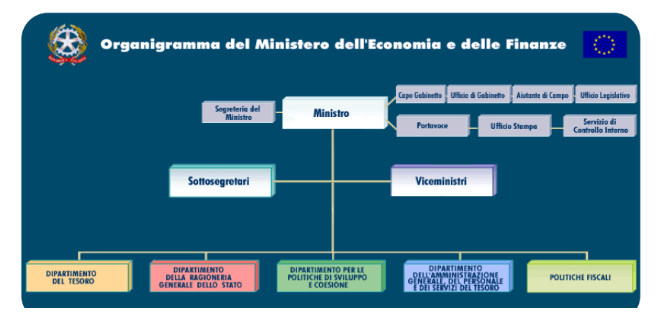
\includegraphics[scale = 0.80]{images/Esempio_Organigramma}
    Esempio di un organigramma 
\end{center}
Questo tipo di rappresentazione grafica ha però dei difetti, in quanto si fa
difficoltà a capire l'importanza delle posizioni rappresentate, non si hanno
informazioni sui rapporti non gerarchici e non si capisce in che ambiente opera
l'azienda.

\subsection{I vari Tipi di Struttura Organizzativa}
\subsubsection{Il modello Gerarchico (Struttura Monofunzionale)}

\begin{center}
    \textcolor{red!50}{CARATTERISTICHE}
\end{center}


\begin{itemize}
    \item \textbf{Principio di gerarchia}, secondo il quale \\ autorità,
    responsabilità e le competenze sono massime al vertice dell'organizzazione;
    \item \textbf{Principio di delega}, secondo il quale le funzioni vengono
    delegate verso il basso;
    \item \textbf{Principio di eccezione}, secondo il quale, in caso di
    difficoltà impreviste il problema deve tornare al vertice per essere
    risolto;
    \item \textbf{Principio dell'unità di direzione}, secondo il quale ciascuno
    deve aver ben chiaro da chi prendere ordini e a chi rivolgersi quando non
    sia in grado di decidere da solo.  
\end{itemize}

\begin{center}
    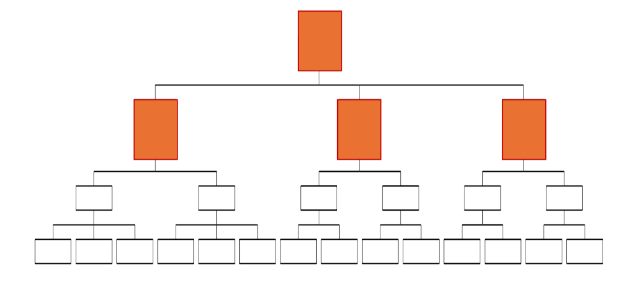
\includegraphics[scale = 0.80]{images/modello_gerarchico}
    Esempio di modello gerarchico
\end{center}

\newpage

\subsubsection{Il modello Gerarchico Funzionale (Struttura Gerarchico Funzionale)}

\begin{center}
    \textcolor{red!50}{CARATTERISTICHE}
\end{center}

Questo modello presenta attività raggruppate in base ad una funzione comune ed
esalta il \textbf{principio della specializzazione} delle singole aree.

Continua a seguire il \textbf{Principio di gerarchia} ed il \textbf{Principio di
eccezione} dal modello precedente.

\begin{center}
    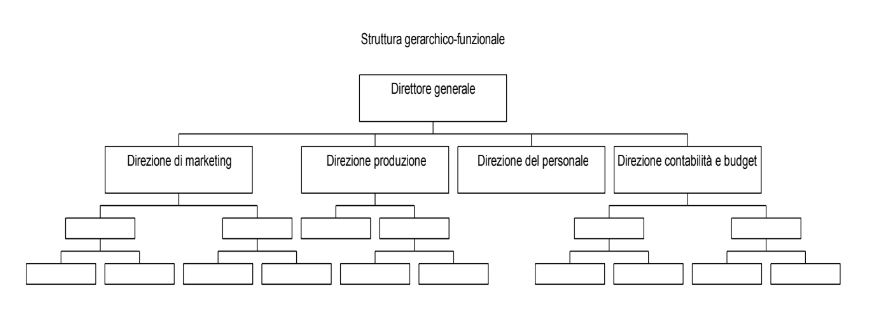
\includegraphics[scale = 0.64]{images/modello_gerarchico_funzionale}
    Esempio di modello gerarchico funzionale
\end{center}
Nella struttura gerarchico funzionale esistono tre livelli organizzativi
fondamentali:

\begin{enumerate}
    \item \textbf{Direzione generale}, a cui è affidato il compito di
    amministrare l'azienda tramite una visione d'insieme che permetta di
    definire gli obiettivi primari e coordinare le diverse aree funzionali;
    \item \textbf{Direzioni dei dipartimenti funzionali}, che sono specializzate
    nelle varie funzioni, quindi non in grado di occuparsi di problemi generali,
    ma solo di problemi settoriali;
    \item \textbf{Unità operative}, ovvero organi che fanno capo ai dipartimenti
    funzionali, per realizzare piani predisposti da quest'ultimi, hanno compiti
    prevalentemente esecutivi. 
\end{enumerate}

Le principali direzioni funzionali sono:

\begin{itemize}
    \item \textbf{Direzione Marketing};
    \item \textbf{Direzione della Produzione};
    \item \textbf{Direzione del Personale};
    \item \textbf{Direzione Amministrativa};
    \item \textbf{Direzione Finanza};
    \item \textbf{Direzione Ricerca e Sviluppo};
\end{itemize}

un esempio di modello gerarchico funzionale può essere identificato nel modello
strutturale utilizzato da Apple.

\subsubsection{Il modello Divisionale}

In questo modello vengono organizzate divisioni separate, ciascuna è
responsabile di un singolo prodotto, servizio o programma principale. Questa
struttura è anche denominata \textbf{struttura per prodotto}.

\begin{center}
    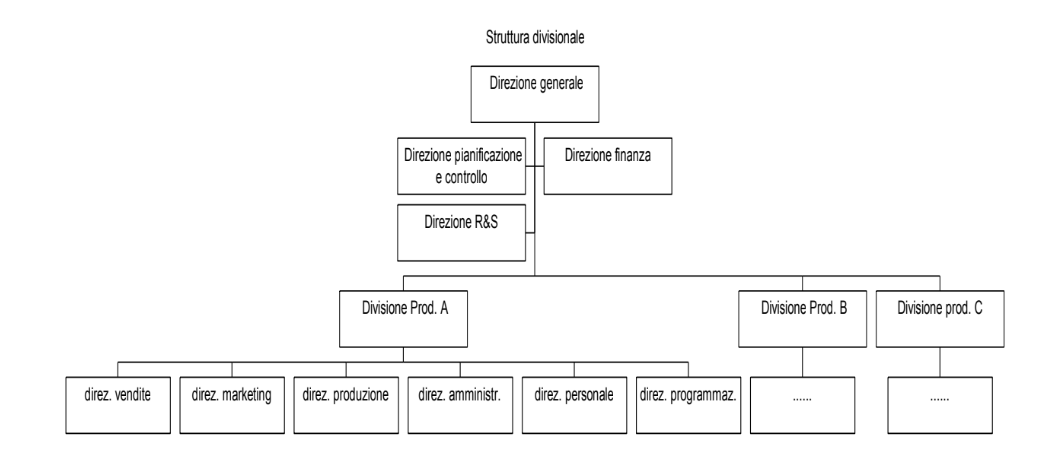
\includegraphics[scale = 0.50]{images/modello_divisionale.png}
    Esempio di modello divisionale
\end{center}

Un'azienda che adopera il modello divisionale è \textbf{Alphabet}, proprietaria
di Google.

\subsubsection{Il modello per Area Geografica}

Questo modello risulta simile al modello divisionale, con l'unica differenza che
le divisioni sono organizzate per area geografica. Questo tipo di struttura
aiuta l'azienda ad espandersi in nuovi mercati e a fare un uso più efficiente
delle risorse.

\begin{center}
    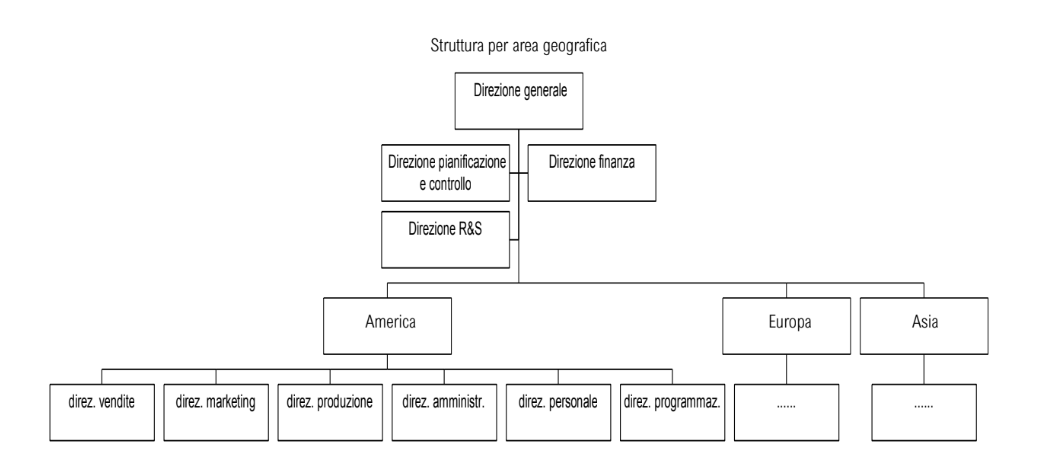
\includegraphics[scale=0.50]{images/modello_geografico.png}
    Esempio di modello per area geografica
\end{center}

\subsubsection{Il modello a Matrice}

Questo modello cerca di combinare al meglio i vantaggi dell' \\ 
organizzazione per funzioni con quelli dell'organizzazione per prodotti o
progetti.

\begin{center}
    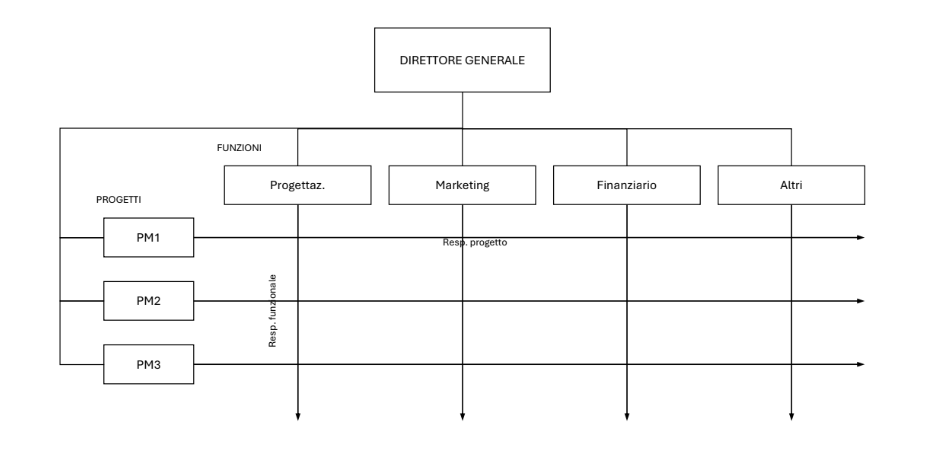
\includegraphics[scale=0.60]{images/modello_matrice.png}
    Esempio di modello a matrice
\end{center}
Molte aziende adoperano questo tipo di struttura, tra le più celebri troviamo
Intel, Spotify, Microsoft, IBM, Philips.

\subsubsection{Il modello a Rete}

Questo modello affida varie parti dell'organizzazione a partner esterni. In
questo caso si parla di \textbf{Outsourcing}, ovvero quando l'azienda ricorre a
fornitori esterni per determinati compiti o funzioni, quali la produzione, le
risorse umane o la gestione dei crediti.

\begin{center}
    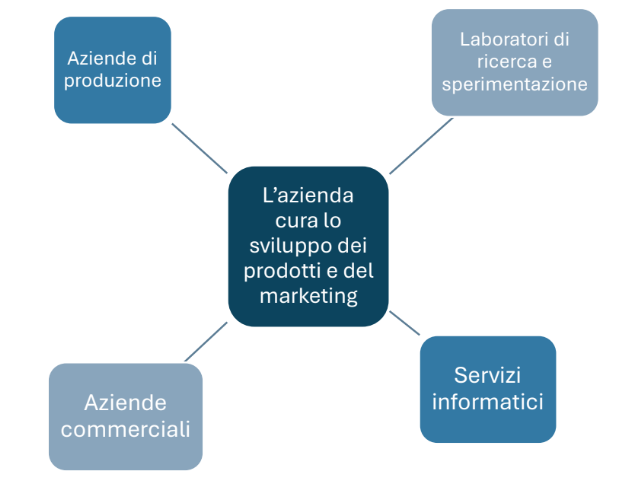
\includegraphics[scale=0.80]{images/modello_rete.png}
\end{center}
Un grande esempio di azienda che adopera questa struttura è Nike, che affida la produzione e la
distribuzione dei propri prodotti ad aziende esterne.

\section{Lezione 4}

\end{document}